\documentclass[a4paper,german,12pt,smallheadings]{scrartcl}
\usepackage[T1]{fontenc}
\usepackage[utf8]{inputenc}
\usepackage{babel}
\usepackage{tikz}
\usepackage{geometry}
\usepackage{amsmath}
\usepackage{amssymb}
\usepackage{float}
\usepackage[thinspace,thinqspace,squaren,textstyle]{SIunits}
\restylefloat{table}
\geometry{a4paper, top=15mm, left=20mm, right=40mm, bottom=20mm, headsep=10mm, footskip=12mm}
\linespread{1.5}
\setlength\parindent{0pt}
\begin{document}
\begin{center}
\bfseries % Fettdruck einschalten
\sffamily % Serifenlose Schrift
\vspace{-40pt}
Analytische Mechanik, Sommersemester 2013, 4. Blatt \\
Luis Herrmann und Markus Fenske, Tutor: Clemens Meyer zu Rheda
\vspace{-10pt}
\end{center}
\section*{Aufgabe 1}

Wir gehen hier von einer Rotation um die x-Achse aus, während in der
Aufgabenstellung eine Rotation um die y-Achse gegeben ist. Die Probleme sind
äquivalent. Wir ermitteln zuerst die minimale Funktion für eine Rotation um die
x-Achse und bilden dann die Umkehrfunktion.

%\resizebox{10cm}{10cm}{%
\begin{figure}[H]
  \begin{center}
    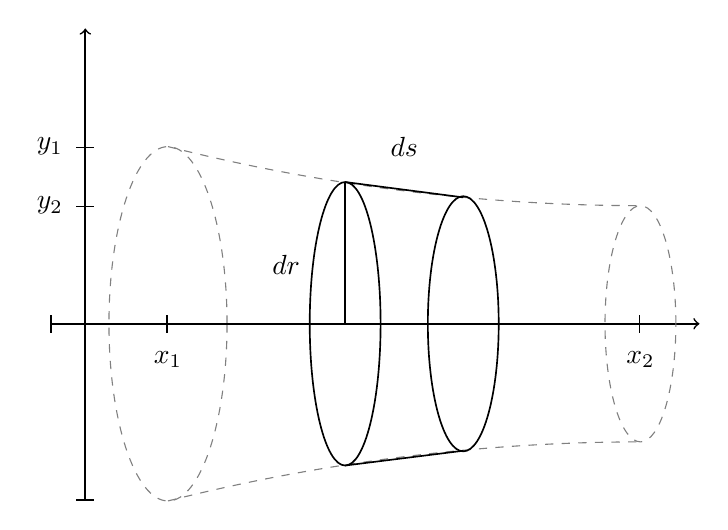
\begin{tikzpicture}[scale=1.5]
      \draw[dashed,color=gray] (0,1.5) ellipse (0.5 and 1.5);% right half of the left ellipse
      \draw[dashed,color=gray] (0,0) parabola bend (4,0.5) (4,0.5);% bottom line
      \draw[dashed,color=gray] (0,3) parabola bend (4,2.5) (4,2.5);% top line
      \draw[semithick] (1.5,1.5) ellipse (0.3 and 1.2);% left du
      \draw[-,semithick] (1.5,2.7) -- (2.5,2.57);
      \draw[-,semithick] (1.5,1.5) -- (1.5,2.7); % dr
      \draw (1.0,2) node {$dr$};
      \draw (2.0,3) node {$ds$};
      \draw[semithick] (2.5,1.5) ellipse (0.3 and 1.08);% left du
      \draw[-,semithick] (1.5,0.3) -- (2.5,0.425); % bottom ds
      \draw[|-|,semithick] (-1,1.5) -- (0,1.5);
      \draw[-|,semithick] (0,1.5) -- (4,1.5);
      \draw[->,semithick] (4,1.5) -- (4.5,1.5);
      \draw[|-|,semithick] (-0.7,0) -- (-0.7,2.5);
      \draw[-|,semithick] (-0.7,2.5) -- (-0.7,3);
      \draw[->,semithick] (-0.7,3) -- (-0.7,4);
      \draw (-1,2.5) node {$y_2$};
      \draw (-1,3) node {$y_1$};
      \draw[dashed,color=gray] (4,1.5) ellipse (0.3 and 1);% right ellipse
      \draw (0,1.2) node {$x_1$};
      \draw (4,1.2) node {$x_2$};
    \end{tikzpicture}
  \end{center}
  \caption{Rotationskörper mit Radiuselement $dr$ und Linienelement $ds$}
\end{figure}
%}

Der Abstand zwischen den Punkten P1 und P2 über die Kurve beträgt:
\begin{equation}
S=\int\limits_S\ ds
\end{equation}
Dabei ist das Wegelement $ds$:
\begin{equation}
ds=\sqrt{dx^2+dy^2}=dx\sqrt{1+\dot{y}^2} \quad mit \quad \dot{y}=\frac{\partial y}{\partial x}
\end{equation}
Für die Rotationsoberfläche gilt:
\begin{equation}
O=\int\limits_O dO \quad wobei \quad dO=2\pi x ds
\end{equation}
Unter Verwendung vom zuvor gefundenen Ausdruck für ds (3) erhalten wir:
\begin{equation}
O=\int\limits_{x_1}^{x_2} 2\pi x \sqrt{1+\dot{y}^2} \; dx = O=2\pi \int\limits_{x_1}^{x_2} x \sqrt{1+\dot{y}^2} \; dx
\end{equation}
Wobei O extremal, genauer gesagt minimal werden soll. Dieses Problem ist äquivalent zu einer Formulierung über die Euler-Lagrange-Gleichung:
\begin{equation}
\frac{d}{dx}\left(\frac{\partial \mathcal{F}}{\partial \dot{y}}\right)-\frac{\partial \mathcal{F}}{\partial y}=0 \quad mit \quad \mathcal{F}(x,y,\dot{y})
\end{equation}
In diesem Fall ist:
\begin{equation}
\mathcal{F}=x \sqrt{1+\dot{y}^2}
\end{equation}
Wir bilden also:
\begin{equation}
\frac{\partial \mathcal{F}}{\partial y}=\frac{\partial x \sqrt{1+\dot{y}^2}}{\partial y}=0
\end{equation}
Da weder $x$ noch $\dot{y}$ explizit von $y$ abhängen.
\begin{equation}
\frac{\partial \mathcal{F}}{\partial \dot{y}}=\frac{\partial x \sqrt{1+ \dot{y}^2}}{\partial \dot{y}}=0 + \frac{2x \dot{y}}{2 \sqrt{1+ \dot{y}^2}}=\frac{x \dot{y}}{\sqrt{1+ \dot{y}^2}}
\end{equation}
Setzen wir (7) und (8) in (5) ein, so erhalten wir:
\begin{align*}
\frac{d}{dx}\left(\frac{x \dot{y}}{\sqrt{1+ \dot{y}^2}}\right)-\frac{\partial x \sqrt{1+\dot{y}^2}}{\partial y}=0\\
\Leftrightarrow \frac{d}{dx}\left(\frac{x \dot{y}}{\sqrt{1+ \dot{y}^2}}\right)-0=0
\end{align*}
Und daraus folgt, dass:
\begin{equation}
\frac{x \dot{y}}{\sqrt{1+ \dot{y}^2}}=const.
\end{equation}
Nennen wir diese Konstante $A$ und formen nach $\dot{y}$ um:
\begin{align*}
\frac{x \dot{y}}{\sqrt{1+ \dot{y}^2}}=A\\
\Leftrightarrow x \dot{y}=A \sqrt{1+\dot{y}^2}\\
\Leftrightarrow x^2 \dot{y}^2=A^2\left(1+\dot{y}^2\right)\\
\Leftrightarrow x^2=A^2 \frac{1+\dot{y}^2}{\dot{y}^2}\\
\Leftrightarrow \frac{x^2}{A^2}=\frac{1}{\dot{y}^2}+1\\
\Leftrightarrow \frac{x^2}{A^2}-1=\frac{1}{\dot{y}^2}\\
\Leftrightarrow \dot{y}^2=\frac{1}{\left(\frac{x^2}{A^2}-1\right)}\\
\Leftrightarrow \dot{y}^2=\frac{A^2}{\left(x^2-A^2\right)}\\
\Leftrightarrow \dot{y}=\frac{A}{\sqrt{x^2-A^2}}
\end{align*}
Damit ist es ein leichtes, die Kurve $y$ auszurechnen:
\begin{equation}
y=\int \dot{y} \; dx=\int \frac{A}{\sqrt{x^2-A^2}} \; dx=A \int \frac{1}{\sqrt{x^2-A^2}} \; dx
\end{equation}
Durch Nachschlagen in der Integraltabelle findet man, dass:
\begin{equation}
\int \frac{1}{\sqrt{x^2-a^2}} \; dx=A sinh\left(\frac{x}{a}\right)
\end{equation}
Und wir erhalten:
\begin{equation}
y=A sinh\left(\frac{x}{A}\right) \quad\\ 
\end{equation}
...mit den Bedingungen:
\begin{equation}
\quad y_1=sinh\left(\frac{x_1}{A}\right) \quad und \quad y_2=sinh\left(\frac{x_2}{A}\right)
\end{equation}

\section*{Aufgabe 2}
\subsection*{Teilaufgabe 1}
Aufstellen der Lagrange-Gleichung 2.Art:
\begin{equation}
V=mgy=mg\left(at+bt^2\right)
\end{equation}
\begin{equation}
T=\frac{m}{2} \dot{y}^2
\end{equation}
Wobei wir den Ansatz verwenden:
\begin{equation}
y=at+bt^2 \Rightarrow \dot{y}=a+2bt \Rightarrow \dot{y}^2=a^2+4abt+4b^2t^2
\end{equation}
Und wir erhalten:
\begin{equation}
\mathcal{L}=T-V=\frac{m}{2} \left(a^2+4abt+4b^2t^2\right) - mg\left(at+bt^2\right)
\end{equation}
\subsection*{Teilaufgabe 2}
Gesucht ist das Ergebnis des Wirkungsintegrals:
\begin{equation}
S=\int\limits_{t_0}^{0} \mathcal{L} \; dt
\end{equation}
Einsetzen der Gleichung aus Teilaufgabe 1 und ausrechnen:
\begin{align*}
S=\int\limits_{0}^{t_0} \frac{m}{2} \left(a^2+4abt+4b^2t^2\right) - mg\left(at+bt^2\right)\\
\Leftrightarrow S=\frac{m}{2} \left(a^2t_0+\frac{4}{3}b^2t_0^3+2abt_0^2\right)-mg\left(\frac{1}{2} at_0^2+ \frac{1}{3} bt_0^3\right)
\end{align*}
\subsection*{Teilaufgabe 3}
Zur Minimierung des Wirkungsintegrals in Abhängigkeit von $a$ und $b$ bilden wir die partiellen Ableitungen nach $a$ und $b$:
\begin{equation}
\frac{\partial S}{\partial a}=\frac{\partial \frac{m}{2} \left(a^2t_0+\frac{4}{3}b^2t_0^3+2abt_0^2\right)-mg\left(\frac{1}{2} at_0^2+ \frac{1}{3} bt_0^3\right)}{\partial a}=\frac{m}{2}\left(2at_0+2bt_0^2\right)-\frac{mgt_0^2}{2}=0
\end{equation}
\\
\begin{equation}
\frac{\partial S}{\partial b}=\frac{\partial \frac{m}{2} \left(a^2t_0+\frac{4}{3}b^2t_0^3+2abt_0^2\right)-mg\left(\frac{1}{2} at_0^2+ \frac{1}{3} bt_0^3\right)}{\partial b}=\frac{m}{2}\left(\frac{8}{3}bt_0^3+2at_0^2\right)-\frac{mgt_0^3}{3}=0
\end{equation}
Gesucht ist die Lösung des linearen Gleichungssystems:
\begin{align*}
a+bt_0-\frac{gt_0}{2}=0\\
\frac{4}{3}bt_0+a-\frac{gt_0}{3}=0\\
\\
\Leftrightarrow a=\frac{gt_0}{2}-bt_0\\
\Leftrightarrow \frac{4}{3}bt_0+\frac{gt_0}{2}-bt_0-\frac{gt_0}{3}=0\\
\\
\Leftrightarrow a=\frac{gt_0}{2}-bt_0\\
\Leftrightarrow \frac{1}{3}bt_0+\frac{1}{6}gt=0\\
\\
\Leftrightarrow a=\frac{gt_0}{2}--\frac{1}{2}gt_0=0\\
\Leftrightarrow b=-\frac{1}{2}g\\
\\
\end{align*}
Und erhalten somit, dass das Wirkungsintegral extremal wird für:
\begin{equation}
y=-\frac{gt^2}{2}
\end{equation}
Wir prüfen, ob es maximal oder minimal wird:
\begin{align*}
\frac{\partial^2 S}{\partial a^2}=\frac{\partial \frac{m}{2}\left(2at_0+2bt_0^2\right)-\frac{mgt_0^2}{2}}{\partial a}=\frac{m}{2}\left(2t_0\right)=mt_0=m \sqrt{\frac{2y_0}{g}}>0
\end{align*}
...da wir $y_0$ und $g$ als positiv definieren.
\begin{align*}
\frac{\partial^2 S}{\partial b^2}=\frac{\partial \frac{m}{2}\left(\frac{8}{3}bt_0^3+2at_0^2\right)-\frac{mgt_0^3}{3}}{\partial b}=\frac{m}{2}\left(\frac{8}{3}t_0^3\right)=\frac{4m}{3} \left(\frac{2y_0}{g}\right)^{3/2}>0
\end{align*}
...siehe oben. Tatsächlich wird das Wirkungsintegral also minimal für:
\begin{equation}
y=-\frac{gt^2}{2}
\end{equation}
\\
\section*{Aufgabe 3}
\subsection*{Teilaufgabe 1}
Die Zwangsbedingungen lauten:
\begin{align}
\tan\alpha=\frac{y_2}{x_1-x_2} \quad \Leftrightarrow \quad y_2=\tan\alpha \left(x_1-x_2\right) \quad \Rightarrow \quad f_1=y_2-\tan\alpha \left(x_1-x_2\right)=0
\end{align}







\end{document}
